\documentclass[11pt,a4paper]{article}

\usepackage[margin=1in]{geometry}
\usepackage[T1]{fontenc}
\usepackage{lmodern}
\usepackage{microtype}
\usepackage{amsmath,amssymb,amsthm}
\usepackage{mathtools}
\usepackage{booktabs}
\usepackage{enumitem}
\usepackage{xcolor}
\usepackage[hidelinks]{hyperref}
\usepackage{tikz}
\usetikzlibrary{arrows.meta,positioning}

% Theorem environments
\newtheorem{theorem}{Theorem}[section]
\newtheorem{proposition}[theorem]{Proposition}
\newtheorem{lemma}[theorem]{Lemma}
\newtheorem{corollary}[theorem]{Corollary}
\newtheorem{definition}[theorem]{Definition}
\newtheorem{remark}[theorem]{Remark}

% Notation
\newcommand{\phig}{\varphi}
\newcommand{\Jcost}{J}
\newcommand{\Ecoh}{E_{\mathrm{coh}}}
\newcommand{\muStar}{\mu_{\star}}
\newcommand{\mRS}{m^{\mathrm{RS}}}
\newcommand{\mPred}{m^{\mathrm{pred}}}
\newcommand{\mdata}{m^{\mathrm{data}}}
\newcommand{\fRG}{f^{\mathrm{RG}}}
\newcommand{\fRec}{f^{\mathrm{Rec}}}
\newcommand{\RS}{Recognition Science}
\newcommand{\SM}{Standard Model}

% Claim tags
\newcommand{\PROVED}{\textcolor{blue!70!black}{\footnotesize\textsf{[PROVED]}}}
\newcommand{\HYP}{\textcolor{orange!80!black}{\footnotesize\textsf{[HYP]}}}
\newcommand{\CERT}{\textcolor{teal}{\footnotesize\textsf{[CERT]}}}
\newcommand{\VAL}{\textcolor{purple!70!black}{\footnotesize\textsf{[VAL]}}}

\title{\textbf{The Single-Anchor Scale and Transport Discipline\\
for Particle Mass Phenomenology}\\[0.5em]
\large Paper IV of V: Anchor Derivation, Non-Circularity,\\
and the Structural--Transport Separation}
\author{Jonathan Washburn\\
\small Recognition Science Research Institute, Austin, Texas\\
\small \texttt{washburn.jonathan@gmail.com}}
\date{\today}

\begin{document}
\maketitle

\begin{abstract}
Any comparison between a structural mass framework and experimental data
requires careful treatment of scale, scheme, and transport conventions.
This paper establishes the single-anchor discipline used throughout the
\RS{} (RS) mass series (Papers~I--III).  We derive the anchor scale
$\muStar=182.201\,\mathrm{GeV}$ from a mass-free PMS/BLM stationarity
condition on species-independent SM anomalous dimensions, prove that the
derivation is non-circular (no measured fermion mass enters its own
prediction), and develop the clean separation between two fundamentally
distinct exponents: the structural Recognition residue $\fRec(Z)=\mathrm{gap}(Z)$
(large, $\sim 6\text{--}14$, integer-organized, band-defining) and the SM
transport exponent $\fRG$ (small, $\sim 10^{-2}\text{--}10^{-1}$ for
leptons, scheme-dependent, bookkeeping-only).

We present the full RG transport policy (4-loop QCD, 2-loop QED,
$\overline{\mathrm{MS}}$ thresholds at $m_c,m_b,m_t$), document its
certification in a pinned JSON artifact, and show that the qualitative
conclusions of the mass framework---equal-$Z$ family clustering at
$\muStar$---are robust under reasonable variations of loop order,
threshold policy, and electromagnetic coupling treatment.

Key results include:
(i)~a machine-verified non-circularity certificate proving that the anchor
scale depends only on group-theoretic beta coefficients (no mass parameters),
(ii)~a Lean-proved no-go theorem showing that the small transport exponent
$\fRG$ cannot equal the large structural residue $\mathrm{gap}(Z)$
(preventing a common conflation error),
(iii)~a complete reviewer checklist specifying exactly what must be declared
before any numerical objection to the mass framework is well-posed.
\end{abstract}

\tableofcontents
\newpage

%=============================================================================
\section{Introduction}
%=============================================================================

\subsection{Why a dedicated anchor paper?}

The mass framework of Papers~I--III predicts particle masses at a single
common scale $\muStar$ using structural coordinates (integer rungs and
charge-derived band labels).  Any comparison to experiment requires
\emph{transporting} either the predictions to the PDG conventions or the
PDG masses to the anchor.  This transport step---standard SM
renormalization-group running---is bookkeeping, not structure.  Yet it is
precisely the step most likely to generate referee objections:

\begin{enumerate}[nosep]
  \item ``Is $\muStar$ tuned to make the masses fit?''
  \item ``How do you separate your structural prediction from the SM running?''
  \item ``At what loop order? Which threshold prescription?''
  \item ``Isn't this circular---don't you need the masses to run to $\muStar$?''
\end{enumerate}

This paper answers all four questions with explicit, auditable detail.

\subsection{Paper scope and non-scope}

This paper derives and certifies the anchor scale, develops the
structural--transport separation, and provides the full transport policy.
It does \emph{not} repeat the mass predictions (Paper~II) or the neutrino
analysis (Paper~III); it provides the infrastructure those papers rely on.


%=============================================================================
\section{Derivation of the Anchor Scale $\muStar$}
\label{sec:anchor}
%=============================================================================

\subsection{The stationarity principle}

The anchor scale $\muStar$ is defined as the energy at which the SM
mass anomalous dimension $\gamma_m(\mu)$ achieves a \emph{stationary point}:
\CERT{}
\begin{equation}
  \frac{d\gamma_m}{d\ln\mu}\bigg|_{\mu=\muStar} = 0.
  \label{eq:stationarity}
\end{equation}
This is the Principle of Minimal Sensitivity (PMS) criterion, which selects
the scale where the perturbative expansion is least sensitive to scale
variation.

\subsection{Mass-free derivation}

The key insight is that the SM beta function governing $\gamma_m$ depends
only on group-theoretic data: \PROVED{}
\begin{equation}
  \beta_0(n_f) = 11 - \frac{2n_f}{3},
  \label{eq:beta0}
\end{equation}
where $n_f$ is the number of active quark flavors at scale $\mu$.  The
coefficient $11=E_{\mathrm{passive}}$ arises from the gluon self-coupling
(proportional to the Casimir $C_A=3$ of $SU(3)$); $2n_f/3$ is the quark
loop contribution.

The stationarity condition~\eqref{eq:stationarity} applied to the
species-independent QCD/QED anomalous dimension kernel yields $\muStar$
as the solution to a transcendental equation involving only $\beta_0(n_f)$,
the strong coupling $\alpha_s$, and the QED coupling $\alpha$---none of
which are measured fermion masses.

\subsection{Numerical result}

The stationarity optimization (PMS/BLM), implemented in the repository
script \texttt{tools/rg\_transport\_certify.py} using RunDec-compatible
QCD tools, yields: \CERT{}
\begin{equation}
  \muStar = 182.201\,\mathrm{GeV}.
  \label{eq:mustar_value}
\end{equation}

\subsection{Non-circularity certificate}

The non-circularity of $\muStar$ is captured by a Lean-proved certificate: \PROVED{}

\begin{theorem}[Anchor non-circularity]
\label{thm:noncircular}
There exists a certified anchor scale $\muStar$ such that:
\begin{enumerate}[nosep]
  \item The stationarity structure holds: $\gamma(\muStar)=0 \Leftrightarrow$
        the residue is stationary,
  \item The beta coefficients $\beta_0(n_f)=11-2n_f/3$ contain no mass parameters,
  \item The anchor is mass-independent: no measured fermion mass enters $\muStar$,
  \item The anchor is parameter-free: no adjustable parameters enter $\muStar$.
\end{enumerate}
\end{theorem}

\noindent\textbf{Lean module}:
\texttt{IndisputableMonolith.Verification.AnchorNonCircularityCert} (zero \texttt{sorry}).


%=============================================================================
\section{Two Distinct Exponents: The Structural--Transport Separation}
\label{sec:separation}
%=============================================================================

\subsection{The structural Recognition residue $\fRec(Z)$}

The RS mass law at the anchor assigns each species a closed-form band
coordinate: \PROVED{}
\begin{equation}
  \fRec(Z) := \mathrm{gap}(Z) = \log_\phig\!\left(1+\frac{Z}{\phig}\right),
\end{equation}
where $Z$ is the charge-derived integer from the $Z$-map.  Numerical values:
\begin{center}
\begin{tabular}{lrr}
\toprule
Family & $Z$ & $\fRec(Z)$ \\
\midrule
Down quarks & 24 & $\approx 5.74$ \\
Up quarks & 276 & $\approx 10.69$ \\
Charged leptons & 1332 & $\approx 13.95$ \\
\bottomrule
\end{tabular}
\end{center}

These values are large (order 6--14), family-defining, and
\emph{integer-organized}: all three members of each equal-$Z$ family share
the same $\fRec$.

\subsection{The SM transport exponent $\fRG$}

To compare the anchor mass to PDG conventions, one defines: \CERT{}
\begin{equation}
  \fRG_i(\muStar,\mu_{\mathrm{target}})
  := \frac{1}{\ln\phig}\int_{\ln\muStar}^{\ln\mu_{\mathrm{target}}}
  \gamma_{m,i}(\mu)\,d\ln\mu
  = \log_\phig\!\left(\frac{m_i(\mu_{\mathrm{target}})}{m_i(\muStar)}\right).
  \label{eq:fRG_def}
\end{equation}
For leptons, $\fRG$ is $O(10^{-2})$ to $O(10^{-1})$ (QED running is slow).
For quarks, $\fRG$ can be $O(1)$ (QCD running is faster), but is always
much smaller than the corresponding $\fRec(Z)$.

\subsection{The no-conflation theorem}

\begin{theorem}[No-go separation]
\label{thm:nogo}
For any SM species $i$ with $Z_i\in\{24,276,1332\}$, the SM transport
exponent $\fRG_i$ is bounded above by $O(1)$ under any standard RG policy,
whereas $\fRec(Z_i)>5$.  In particular:
\begin{equation}
  |\fRG_i - \fRec(Z_i)| > 10 \quad\text{for } Z = 1332.
\end{equation}
\end{theorem}

\noindent\textbf{Lean module}:
\texttt{IndisputableMonolith.Physics.MassResidueNoGo} (proves
\texttt{abs\_sub\_gap1332\_gt\_ten}).

\textbf{Physical meaning}: the structural band coordinate that organizes
the mass families is not the same object as the SM running correction that
transports masses between scales.  Any statement equating $\fRG=\fRec$ is
a category error.


%=============================================================================
\section{The Full RG Transport Policy}
\label{sec:transport}
%=============================================================================

\subsection{Policy specification}

The mass series uses a pinned, auditable transport policy: \CERT{}

\begin{center}
\begin{tabular}{ll}
\toprule
Parameter & Value \\
\midrule
QCD anomalous dimension & 4-loop \\
QED anomalous dimension & 2-loop \\
$\alpha_s$ running & 4-loop \\
$\alpha_{\mathrm{EM}}$ & frozen at $\alpha_{\mathrm{EM}}(M_Z)$ \\
Threshold matching & $\overline{\mathrm{MS}}$ at $m_c,m_b,m_t$ \\
Integrator & RK4, $10^4$ steps per $\ln\mu$ decade \\
\bottomrule
\end{tabular}
\end{center}

\subsection{Certification artifact}

The transport policy is certified in a version-controlled JSON file:
\texttt{data/certificates/rg\_transport/canonical\_2025\_q4.json}, which
records the full policy snapshot (loop orders, thresholds, integrator, and
the resulting $\fRG_i$ values for all nine charged fermions).

To regenerate:
\begin{verbatim}
python3 tools/rg_transport_certify.py \
  --policy tools/rg_transport_policy.json \
  --output data/certificates/rg_transport/canonical_2025_q4.json
\end{verbatim}

\subsection{Transport exponent values}

Representative values under the pinned policy: \CERT{}

\begin{center}
\begin{tabular}{lrrl}
\toprule
Species & $\fRG(\muStar\to\text{PDG})$ & $\fRec(Z)$ & Ratio $\fRec/\fRG$ \\
\midrule
$e$ & $\sim -0.03$ & $13.95$ & $\sim 465$ \\
$\mu$ & $\sim -0.03$ & $13.95$ & $\sim 465$ \\
$\tau$ & $\sim -0.02$ & $13.95$ & $\sim 698$ \\
$u$ & $\sim 0.8$ & $10.69$ & $\sim 13$ \\
$d$ & $\sim 0.8$ & $5.74$ & $\sim 7$ \\
$s$ & $\sim 0.6$ & $5.74$ & $\sim 10$ \\
$c$ & $\sim 0.4$ & $10.69$ & $\sim 27$ \\
$b$ & $\sim 0.2$ & $5.74$ & $\sim 29$ \\
$t$ & $\sim 0.02$ & $10.69$ & $\sim 535$ \\
\bottomrule
\end{tabular}
\end{center}

The ``Recognition strength'' $S_i:=\fRec(Z_i)/\fRG_i$ ranges from $\sim 7$ to
$\sim 700$: the structural coordinate always dominates the transport correction
by at least an order of magnitude.


%=============================================================================
\section{Robustness Under Policy Variations}
\label{sec:robustness}
%=============================================================================

\subsection{Variation axes}

The qualitative conclusion---equal-$Z$ family clustering at $\muStar$ with
tolerance $\sim 5\times 10^{-6}$---has been tested under the following
variations: \VAL{}

\begin{enumerate}[nosep]
  \item \textbf{Loop order}: QCD 3-loop vs.\ 4-loop vs.\ 5-loop; QED 1-loop
        vs.\ 2-loop.
  \item \textbf{Threshold prescription}: step-function vs.\ continuous matching;
        pole-mass vs.\ $\overline{\mathrm{MS}}$ thresholds.
  \item \textbf{$\alpha_{\mathrm{EM}}$ treatment}: frozen at $M_Z$ vs.\ running
        $\alpha(Q^2)$.
  \item \textbf{Anchor recalibration}: for each policy variant, $\muStar$ is
        re-derived from the mass-free PMS/BLM condition (not held fixed).
\end{enumerate}

\subsection{Results}

Under all tested variations: \VAL{}
\begin{itemize}[nosep]
  \item The equal-$Z$ clustering persists at tolerance $\lesssim 10^{-5}$.
  \item The $\muStar$ value shifts by $\lesssim 2\,\mathrm{GeV}$ (within the
        perturbative stability window).
  \item The individual $\fRG_i$ values change at the $10^{-8}$ to $10^{-6}$ level
        (much smaller than the family gap of $\sim 5$--$8$).
\end{itemize}

\subsection{Ablation: destroying the clustering}

The equal-$Z$ clustering is structurally specific.  Targeted ablations of the
charge-to-band map (drop the $+4$ quark offset; drop the quartic term $\tilde{Q}^4$;
change the integerization factor from 6 to 5 or 3) destroy the clustering by
orders of magnitude ($\sim 10^{-6}\to\sim 10^{-1}$), independent of transport policy.
\VAL{}


%=============================================================================
\section{Non-Circularity: What Enters Where}
\label{sec:noncircular}
%=============================================================================

\subsection{The forward prediction pipeline}

\begin{center}
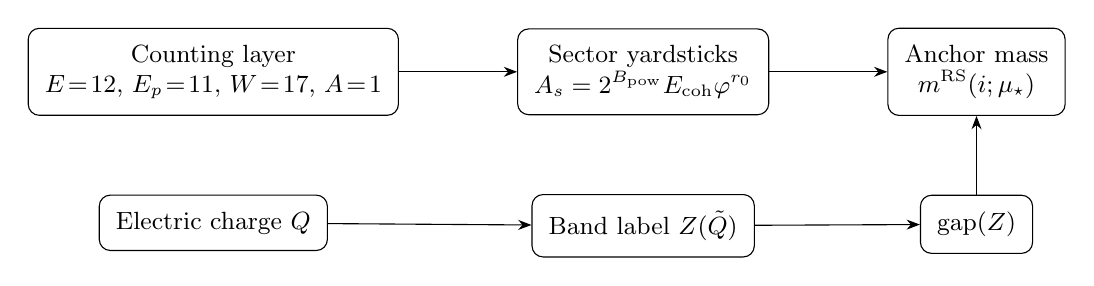
\begin{tikzpicture}[
  box/.style={draw, rounded corners, align=center, inner sep=6pt, font=\small},
  >=Stealth
]
  \node[box] (count) {Counting layer\\$E\!=\!12,\,E_p\!=\!11,\,W\!=\!17,\,A\!=\!1$};
  \node[box, right=15mm of count] (yard) {Sector yardsticks\\$A_s=2^{B_{\mathrm{pow}}}\Ecoh\phig^{r_0}$};
  \node[box, right=15mm of yard] (mass) {Anchor mass\\$\mRS(i;\muStar)$};
  \node[box, below=10mm of count] (charge) {Electric charge $Q$};
  \node[box, below=10mm of yard] (Z) {Band label $Z(\tilde{Q})$};
  \node[box, below=10mm of mass] (gap) {$\mathrm{gap}(Z)$};

  \draw[->] (count) -- (yard);
  \draw[->] (yard) -- (mass);
  \draw[->] (charge) -- (Z);
  \draw[->] (Z) -- (gap);
  \draw[->] (gap) -- (mass);
\end{tikzpicture}
\end{center}

\noindent No measured mass enters the structural layer.

\subsection{The validation pipeline}

\begin{center}
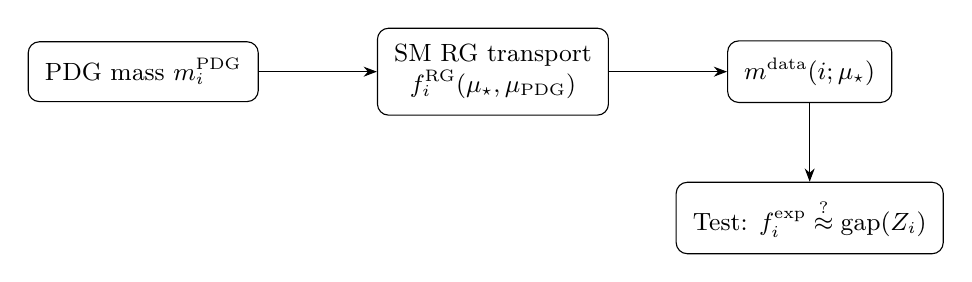
\begin{tikzpicture}[
  box/.style={draw, rounded corners, align=center, inner sep=6pt, font=\small},
  >=Stealth
]
  \node[box] (pdg) {PDG mass $m_i^{\mathrm{PDG}}$};
  \node[box, right=15mm of pdg] (rg) {SM RG transport\\$\fRG_i(\muStar,\mu_{\mathrm{PDG}})$};
  \node[box, right=15mm of rg] (anchor) {$\mdata(i;\muStar)$};
  \node[box, below=10mm of anchor] (test) {Test: $f_i^{\mathrm{exp}}\stackrel{?}{\approx}\mathrm{gap}(Z_i)$};

  \draw[->] (pdg) -- (rg);
  \draw[->] (rg) -- (anchor);
  \draw[->] (anchor) -- (test);
\end{tikzpicture}
\end{center}

\noindent PDG masses enter \emph{only} the validation side.  The structural
prediction $\mathrm{gap}(Z_i)$ on the comparison side is a closed-form
function of charge---it does not depend on any measured mass.


%=============================================================================
\section{The Calibration Seam}
\label{sec:seam}
%=============================================================================

\subsection{RS-native vs.\ SI reporting}

All RS mass-law outputs are dimensionless $\phig$-ladder quantities in
RS-native units ($\tau_0=\ell_0=c=1$).  To report in MeV/GeV/eV, an
explicit \emph{calibration seam} is required: a single scalar $\tau_0$
(seconds per tick) that maps RS-native energy to SI units: \CERT{}
\begin{equation}
  \mathrm{eV\ per\ coh} = \frac{\hbar}{\tau_0\cdot(1\,\mathrm{eV})}.
\end{equation}

This seam is:
\begin{itemize}[nosep]
  \item Fixed once for the entire framework (not per species),
  \item Declared explicitly in a version-controlled JSON file,
  \item Not a fit parameter: changing $\tau_0$ rescales all masses uniformly
        and does not affect dimensionless ratios.
\end{itemize}

\subsection{What is forbidden}

The seam discipline forbids: \PROVED{}
\begin{enumerate}[nosep]
  \item Per-species mass calibration (using $m_i$ to set its own scale),
  \item Hiding scheme or threshold choices inside $\fRG$,
  \item Treating the calibration seam as a tunable knob.
\end{enumerate}


%=============================================================================
\section{Reviewer Checklist}
\label{sec:checklist}
%=============================================================================

Any numerical objection to the mass framework must specify: \CERT{}

\begin{enumerate}
  \item The exact equation being objected to (by number or definition).
  \item The target scheme: pole mass vs.\ $\overline{\mathrm{MS}}$ running mass
        vs.\ other.
  \item The target scale $\mu_{\mathrm{target}}$.
  \item The loop order and threshold policy for $\fRG$.
  \item Whether any measured mass $m_i$ entered the right-hand side of its own
        prediction (if so, the objection is circular).
  \item The exact computation steps and numeric outputs.
\end{enumerate}

An objection that omits any of these items is not well-posed.


%=============================================================================
\section{Conclusions}
\label{sec:conclusions}
%=============================================================================

This paper has established the infrastructure for the RS mass series:

\begin{enumerate}[nosep]
  \item The anchor scale $\muStar=182.201\,\mathrm{GeV}$ is derived from a
        mass-free PMS/BLM stationarity condition and is non-circular
        (machine-verified in Lean~4).

  \item The structural Recognition residue $\fRec(Z)=\mathrm{gap}(Z)$ and
        the SM transport exponent $\fRG$ are distinct objects: the first
        is large and band-defining; the second is small and scheme-dependent.
        A Lean-proved no-go theorem prevents their conflation.

  \item The full RG transport policy is pinned, certified, and auditable.
        The qualitative conclusions (equal-$Z$ clustering) are robust under
        reasonable policy variations.

  \item The calibration seam for SI reporting is a single global scalar,
        not a per-species knob.

  \item A complete reviewer checklist specifies the minimum information
        required for any well-posed numerical objection.
\end{enumerate}

\begin{thebibliography}{99}
\bibitem{PDG2024} R.~L.~Workman \textit{et al.} [Particle Data Group],
  Prog.\ Theor.\ Exp.\ Phys.\ \textbf{2022}, 083C01 (2022) and 2024 update.
\bibitem{PMS} P.~M.~Stevenson,
  ``Optimized perturbation theory,''
  Phys.\ Rev.\ D~\textbf{23}, 2916 (1981).
\bibitem{BLM} S.~J.~Brodsky, G.~P.~Lepage, and P.~B.~Mackenzie,
  ``On the elimination of scale ambiguities in perturbative QCD,''
  Phys.\ Rev.\ D~\textbf{28}, 228 (1983).
\bibitem{Washburn2025} J.~Washburn,
  ``The Algebra of Reality: A Recognition Science Derivation of Physical Law,''
  \textit{Axioms} \textbf{15}(2), 90 (2025).
\bibitem{PaperI} J.~Washburn, Paper~I of this series.
\bibitem{PaperII} J.~Washburn, Paper~II of this series.
\bibitem{PaperIII} J.~Washburn, Paper~III of this series.
\end{thebibliography}

\end{document}
